\documentclass[12pt]{article}
\usepackage[margin=1in]{geometry}

% Font and Language (Computer Modern, xelatex)
\usepackage{polyglossia}
\setmainlanguage{greek}
\setotherlanguage{english}
\newfontfamily\greekfont{FreeSerif}
\newfontfamily\greekfonttt{FreeSerif}

% General
\usepackage{graphicx}
\graphicspath{ {./pictures/} }
\usepackage{caption}
\captionsetup{labelsep=none, font={small,it}}
\renewcommand{\thefigure}{}
\usepackage{float}
\usepackage{ragged2e}
\usepackage{fancyhdr}
\usepackage{titlesec}
\usepackage{xcolor}
\usepackage{minted}
\usepackage{hyperref}
\usepackage{listings}
\usepackage[table]{xcolor}
\arrayrulecolor{black}

% Listings configuration with colors and frame
\lstset{
    backgroundcolor=\color{white},
    frame=single,
    framesep=4pt,
    framerule=0.5pt,
    rulecolor=\color{gray!50},
    basicstyle=\ttfamily\small,
    keywordstyle=\color{blue}\bfseries,
    stringstyle=\color{red},
    commentstyle=\color{green!50!black},
    numberstyle=\tiny\color{gray},
    numbers=left,
    numbersep=5pt,
    stepnumber=1,
    showstringspaces=false,
    tabsize=4,
    breaklines=true,
    breakatwhitespace=false,
    language=VHDL
} 
\hypersetup{
    colorlinks=true,
    linkcolor=blue
}

% Layout
\setlength{\parindent}{0pt}
\setlength{\parskip}{0.5em}

% Title
\title{}
\author{}
\date{}


\begin{document}
    \begin{titlepage}
        \begin{center}
            
            \begin{minipage}{0.3\textwidth}
                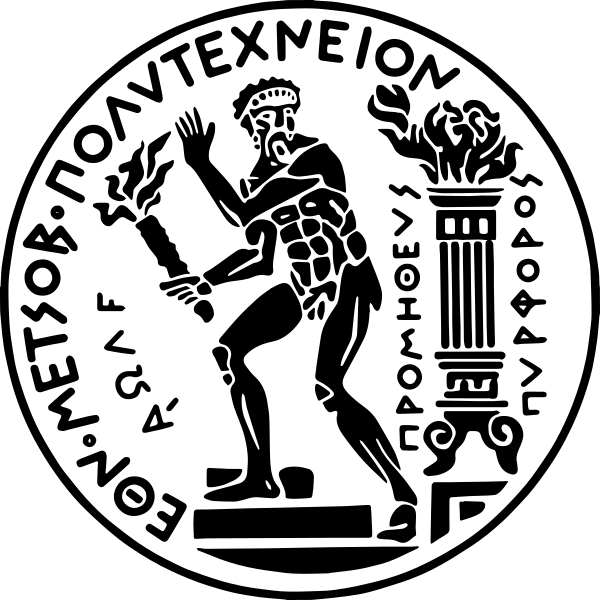
\includegraphics[width=\linewidth]{ntua_logo.png}
            \end{minipage}
            \hfill
            \begin{minipage}{0.65\textwidth}
                \centering
                {\LARGE \textbf{Εθνικό Μετσόβιο Πολυτεχνείο}}\\[0.3cm]
                {\large \textbf{Σχολή Ηλεκτρολόγων Μηχανικών \& Μηχανικών Υπολογιστών}}\\[0.2cm]
                \rule{\linewidth}{0.5pt}\\[0.3cm]
                {\large Εξάμηνο 8\textsuperscript{o}}\\
                {\large \textbf{Ψηφιακά Συστήματα VLSI}}\\
            \end{minipage}
            
            \vspace{2cm}
            
            {\Huge \textbf{1η Εργαστηριακή Άσκηση}}\\[1 cm]
            
            {\Large \textbf{Υλοποίηση Βασικών Ψηφιακών Κυκλωμάτων σε VHDL}}\\[5 cm]
            
            {\Large \textbf{Μέλη Ομάδας}}\\[0.5cm]
            
            \begin{tabular}{rl}
                \textbf{Καβαδάκης Σωτήρης} & 03122035 \\
                \textbf{Κοντοπίδης Δημήτρης} & 03122025 \\
            \end{tabular}
            
            \vfill
            
            {\large Αθήνα, Μάρτιος 2026}
            
        \end{center}
    \end{titlepage}
    \clearpage

% ==============================================================================
% ΜΕΡΟΣ Α
% ==============================================================================
\newpage
\section*{Μέρος Α}
\addcontentsline{toc}{section}{Μέρος Α}

% ------------------------------------------------------------------------------
% Α.2 Decoder 3-to-8
% ------------------------------------------------------------------------------
\section*{Α.2 Decoder 3-to-8}
\addcontentsline{toc}{subsection}{Α.2 Decoder 3-to-8}

\subsection*{Περιγραφή Κυκλώματος}

Ο αποκωδικοποιητής 3-to-8 (Decoder 3 προς 8) είναι ένα συνδυαστικό κύκλωμα που μετατρέπει μια δυαδική είσοδο 3 bits σε μοναδική έξοδο 8 bits. Για κάθε συνδυασμό εισόδου, ακριβώς μία έξοδος είναι ενεργή (λογικό '1'), ενώ οι υπόλοιπες είναι ανενεργές (λογικό '0').

Υλοποιήθηκαν δύο εκδόσεις του κυκλώματος:
\begin{itemize}
    \item \textbf{Behavioral Model}: Χρησιμοποιεί δομή case για περιγραφή της λειτουργίας
    \item \textbf{Dataflow Model}: Χρησιμοποιεί δήλωση with-select για περιγραφή της ροής δεδομένων
\end{itemize}

\subsection*{Σχεδιάγραμμα Λειτουργίας}

\begin{figure}[H]
    \centering
    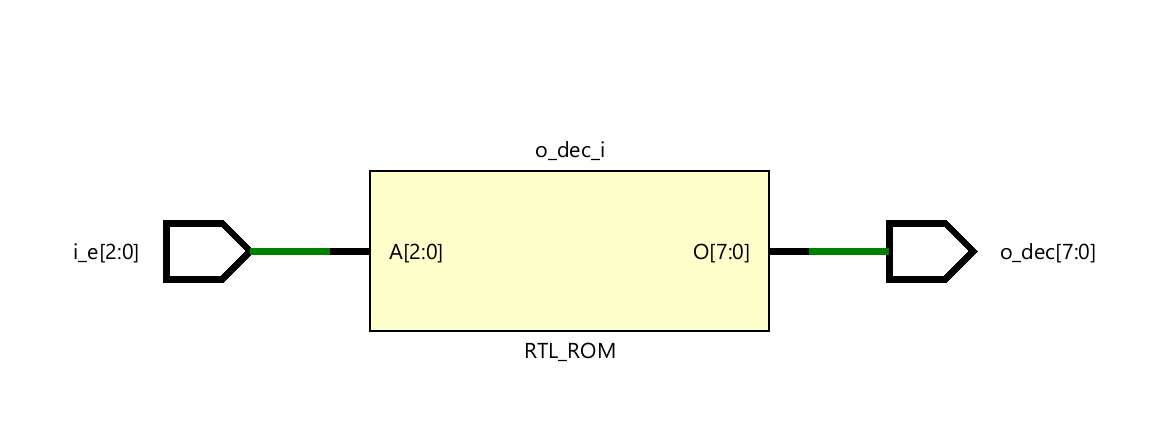
\includegraphics[width=0.7\textwidth]{RTL/decoder.png}
    \caption{RTL σχηματικό του Decoder 3-to-8}
    \label{fig:decoder_rtl}
\end{figure}

Ο πίνακας αλήθειας του Decoder 3-to-8:

\begin{table}[H]
    \centering
    \begin{tabular}{|c|c|}
        \hline
        \textbf{Είσοδος (i\_e)} & \textbf{Έξοδος (o\_dec)} \\
        \hline
        000 & 00000001 \\
        \hline
        001 & 00000010 \\
        \hline
        010 & 00000100 \\
        \hline
        011 & 00001000 \\
        \hline
        100 & 00010000 \\
        \hline
        101 & 00100000 \\
        \hline
        110 & 01000000 \\
        \hline
        111 & 10000000 \\
        \hline
    \end{tabular}
    \caption{Πίνακας αλήθειας Decoder 3-to-8}
    \label{tab:decoder_truth}
\end{table}

\subsection*{Κώδικας VHDL - Behavioral Model}

\begin{lstlisting}[language=VHDL]
-- 3-to-8 Decoder Behavioral Model

library IEEE;
use IEEE.std_logic_1164.all;

entity decoder_3_8_bh is
    port(
    a : in std_logic_vector(2 downto 0);
    y : out std_logic_vector(7 downto 0));
end;

architecture behavioral of decoder_3_8_bh is
begin
    process(a)
    begin
        y <= "00000000";
        case a is
            when "000" => y(0) <= '1';
            when "001" => y(1) <= '1';
            when "010" => y(2) <= '1';
            when "011" => y(3) <= '1';
            when "100" => y(4) <= '1';
            when "101" => y(5) <= '1';
            when "110" => y(6) <= '1';
            when "111" => y(7) <= '1';
            when others => null;
        end case;
    end process;
end behavioral;
\end{lstlisting}

\subsection*{Κώδικας VHDL - Dataflow Model}

\begin{lstlisting}[language=VHDL]
-- 3-to-8 Decoder Dataflow Model

library IEEE;
use IEEE.std_logic_1164.all;

entity decoder_3_8_df is
    port(
    a : in std_logic_vector(2 downto 0);
    y : out std_logic_vector(7 downto 0));
end;

architecture dataflow of decoder_3_8_df is
begin
    with a select
        y <= "00000001" when "000",
             "00000010" when "001",
             "00000100" when "010",
             "00001000" when "011",
             "00010000" when "100",
             "00100000" when "101",
             "01000000" when "110",
             "10000000" when "111",
             "00000000" when others;
end dataflow;
\end{lstlisting}

Παρατηρούμε ότι και οι δύο υλοποιήσεις παράγουν το ίδιο αποτέλεσμα στο RTL σχηματικό, πράγμα που σημαίνει ότι το vivado έχει βελτιστοποιήσει την υλοποίηση του κυκλώματος.

\subsection*{Testbench}

\begin{lstlisting}[language=VHDL]
-- 3-to-8 Decoder Testbench

library IEEE;
use IEEE.std_logic_1164.all;

entity decoder3_8_tb is
end entity;

architecture tb of decoder3_8_tb is
    component decoder_3_8_bh is
        port(a : in std_logic_vector(2 downto 0);
             y : out std_logic_vector(7 downto 0));
    end component;
    
    signal a : std_logic_vector(2 downto 0);
    signal y_bh, y_df : std_logic_vector(7 downto 0);
    
begin
    DUT_BH : entity work.decoder_3_8_bh(behavioral)
        port map(a => a, y => y_bh);
    
    DUT_DF : entity work.decoder_3_8_df(dataflow)
        port map(a => a, y => y_df);
    
    stimulus : process
    begin
        for i in 0 to 7 loop
            a <= std_logic_vector(to_unsigned(i, 3));
            wait for 10 ns;
            assert y_bh = y_df report "Mismatch at input " & integer'image(i) severity error;
            assert y_bh = std_logic_vector(to_unsigned(2**i, 8)) 
                report "Expected output mismatch" severity error;
        end loop;
        wait;
    end process;
end tb;
\end{lstlisting}

\subsection*{Ανάλυση Αποτελεσμάτων Testbench}

Το testbench ελέγχει εξαντλητικά όλους τους 8 δυνατούς συνδυασμούς εισόδου (0 έως 7). Για κάθε είσοδο, επαληθεύει ότι η έξοδος αντιστοιχεί στην αναμενόμενη τιμή σύμφωνα με τον πίνακα αλήθειας χρησιμοποιώντας εντολές assert. Εφόσον δεν υπήρχε κάποιο assert error statement κατά την εκτέλεση της προσομοίωσης, επιβεβαιώθηκε η ορθή λειτουργία και των δύο υλοποιήσεων (Behavioral και Dataflow).

% ------------------------------------------------------------------------------
% Μετρητής 3-bit Up/Down
% ------------------------------------------------------------------------------
\newpage
\section*{Β.2 Μετρητής 3-bit Up/Down}
\addcontentsline{toc}{subsection}{β.2 Μετρητής 3-bit Up/Down}

\subsection*{Περιγραφή Κυκλώματος}

Ο μετρητής 3-bit Up/Down είναι ένα ακολουθιακό κύκλωμα που μπορεί να μετράει είτε προς τα πάνω είτε προς τα κάτω, κάθε φορά αλλάζοντας την τιμή του κατά 1. Υλοποιήθηκαν δύο εκδόσεις:

\begin{itemize}
    \item \textbf{RTL No Limit}: Μετράει κυκλικά από 0 έως 7 (για up) ή 7 έως 0 (για down)
    \item \textbf{RTL Limit}: Μετράει μέχρι ένα καθορισμένο όριο (lim) που ορίζεται από τον χρήστη
\end{itemize}

Είσοδοι:
\begin{itemize}
    \item \texttt{up}: Επιλογή κατεύθυνσης ('1' = up, '0' = down)
    \item \texttt{clk}: Σήμα ρολογιού
    \item \texttt{resetn}: Ασύγχρονη επαναφορά (ενεργή σε '0')
    \item \texttt{count\_en}: Ενεργοποίηση μέτρησης
    \item \texttt{lim}: Όριο μέτρησης (μόνο για την έκδοση με όριο)
\end{itemize}

Έξοδοι:
\begin{itemize}
    \item \texttt{sum}: Τρέχουσα τιμή μετρητή (3 bits)
    \item \texttt{cout}: Σήμα υπερχείλισης/κάτω ροής ('1' όταν φτάνει τα όρια)
\end{itemize}

\subsection*{Σχεδιάγραμμα Λειτουργίας}

\begin{figure}[H]
    \centering
    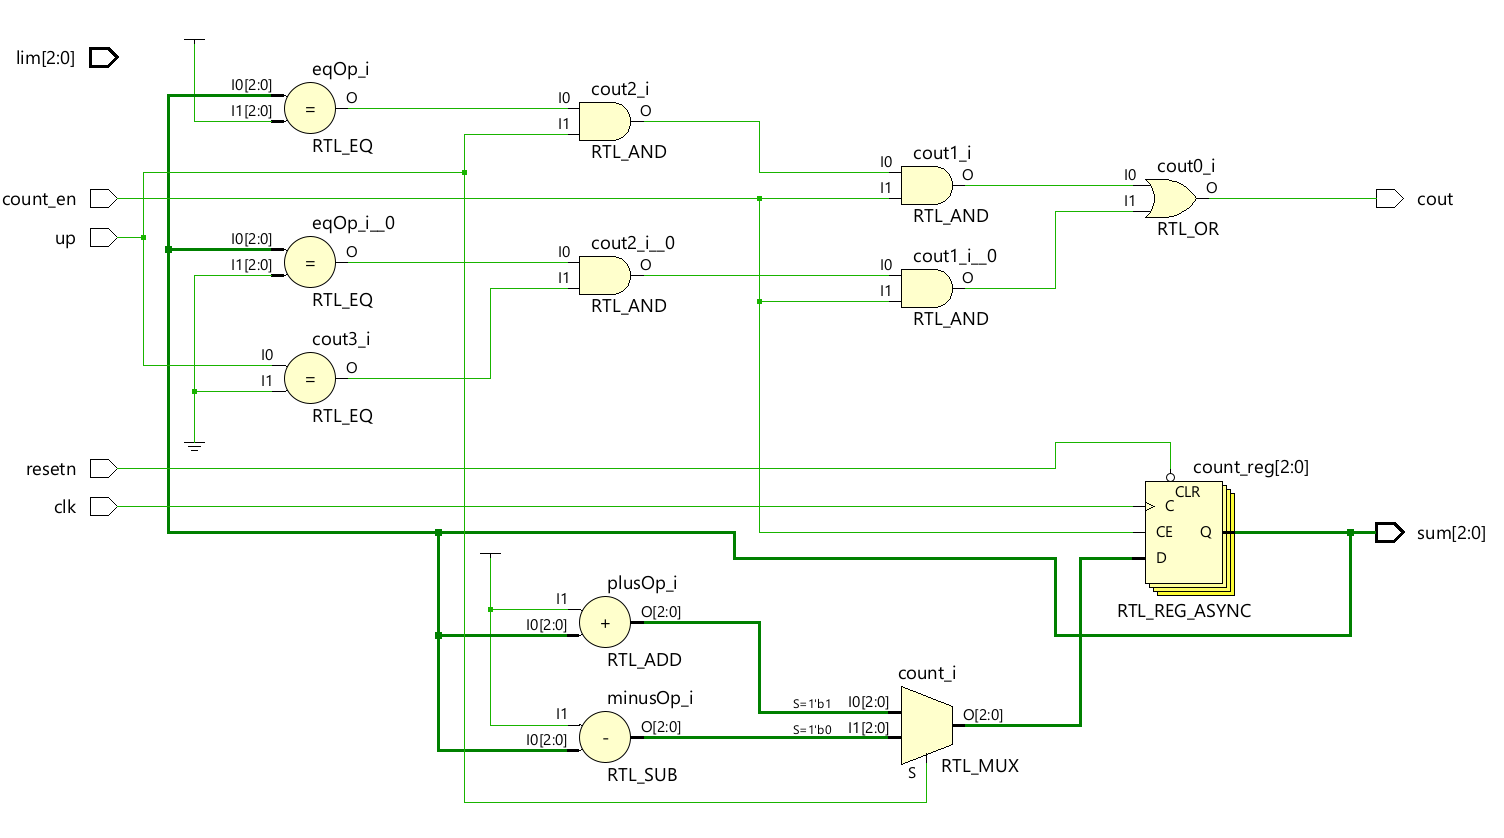
\includegraphics[width=0.9\textwidth]{RTL/counter_nolimit.png}
    \caption{RTL σχηματικό του Μετρητή Up/Down (χωρίς όριο)}
    \label{fig:counter_nolimit_rtl}
\end{figure}

\begin{figure}[H]
    \centering
    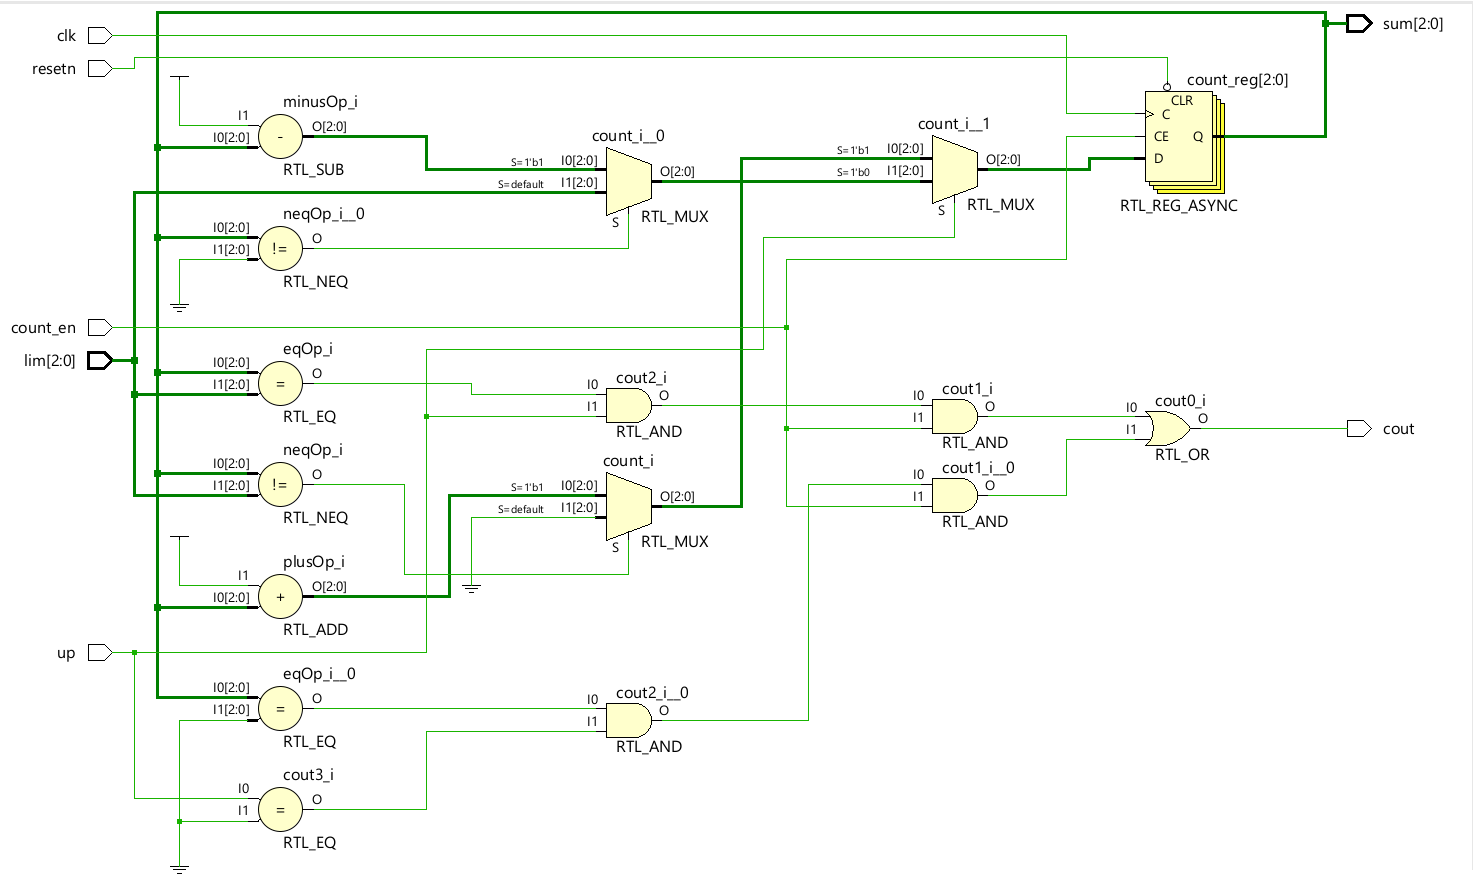
\includegraphics[width=0.9\textwidth]{RTL/counter_limit.png}
    \caption{RTL σχηματικό του Μετρητή Up/Down (με όριο)}
    \label{fig:counter_limit_rtl}
\end{figure}

Η λειτουργία βασίζεται σε 3 flip flops, των οποίων η τιμή μεταβάλλεται στη θετική ακμή του ρολογιού. Συγκεκριμένα, σε κάθε θετική ακμή του ρολογιού, αν η μέτρηση είναι ενεργοποιημένη, η τιμή του μετρητή αυξάνεται ή μειώνεται κατά 1.

\subsection*{Κώδικας VHDL}

\begin{lstlisting}[language=VHDL]
-- 3-bit Up/Down Counter

library IEEE;
use IEEE.std_logic_1164.all;
use IEEE.numeric_std.all;

entity count3_updown is
    port(
        up      : in std_logic;
        clk     : in std_logic;
        resetn  : in std_logic;
        count_en: in std_logic;
        lim     : in std_logic_vector(2 downto 0);
        sum     : out std_logic_vector(2 downto 0);
        cout    : out std_logic
    );
end;

architecture rtl_nolimit of count3_updown is
    signal count : unsigned(2 downto 0);
begin
    process(clk, resetn)
    begin
        if resetn = '0' then
            count <= (others => '0');
        elsif rising_edge(clk) then
            if count_en = '1' then
                if up = '1' then
                    if count = 7 then
                        count <= (others => '0');
                    else
                        count <= count + 1;
                    end if;
                else
                    if count = 0 then
                        count <= to_unsigned(7, 3);
                    else
                        count <= count - 1;
                    end if;
                end if;
            end if;
        end if;
    end process;
    
    sum <= std_logic_vector(count);
    cout <= '1' when (up = '1' and count = 7) or (up = '0' and count = 0) else '0';
end rtl_nolimit;

architecture rtl_limit of count3_updown is
    signal count : unsigned(2 downto 0);
begin
    process(clk, resetn)
    begin
        if resetn = '0' then
            count <= (others => '0');
        elsif rising_edge(clk) then
            if count_en = '1' then
                if up = '1' then
                    if count >= unsigned(lim) then
                        count <= (others => '0');
                    else
                        count <= count + 1;
                    end if;
                else
                    if count = 0 then
                        count <= unsigned(lim);
                    else
                        count <= count - 1;
                    end if;
                end if;
            end if;
        end if;
    end process;
    
    sum <= std_logic_vector(count);
    cout <= '1' when (up = '1' and count = unsigned(lim)) or (up = '0' and count = 0) else '0';
end rtl_limit;
\end{lstlisting}

\subsection*{Testbench}

\begin{lstlisting}[language=VHDL]
-- 3-bit Up/Down Counter Testbench

library IEEE;
use IEEE.std_logic_1164.all;
use IEEE.numeric_std.all;

entity count3_updown_tb is
end entity;

architecture tb of count3_updown_tb is
    component count3_updown is
        port(
            up      : in std_logic;
            clk     : in std_logic;
            resetn  : in std_logic;
            count_en: in std_logic;
            lim     : in std_logic_vector(2 downto 0);
            sum     : out std_logic_vector(2 downto 0);
            cout    : out std_logic
        );
    end component;
    
    signal up      : std_logic := '1';
    signal clk     : std_logic := '0';
    signal resetn  : std_logic := '0';
    signal count_en: std_logic := '0';
    signal lim     : std_logic_vector(2 downto 0) := "101";
    signal sum     : std_logic_vector(2 downto 0);
    signal cout    : std_logic;
    
begin
    clk <= not clk after 5 ns;
    
    DUT_NOLIMIT : entity work.count3_updown(rtl_nolimit)
        port map(up, clk, resetn, count_en, "111", sum, cout);
    
    DUT_LIMIT : entity work.count3_updown(rtl_limit)
        port map(up, clk, resetn, count_en, lim, open, open);
    
    stimulus : process
    begin
        resetn <= '0';
        wait for 20 ns;
        resetn <= '1';
        count_en <= '1';
        
        -- Test count up no limit
        up <= '1';
        wait for 80 ns;
        
        -- Test count down no limit
        up <= '0';
        wait for 80 ns;
        
        -- Test count up with limit
        up <= '1';
        lim <= "101";
        wait for 70 ns;
        
        -- Test count down with limit
        up <= '0';
        wait for 70 ns;
        
        wait;
    end process;
end tb;
\end{lstlisting}

\subsection*{Ανάλυση Αποτελεσμάτων Testbench}

Το testbench ελέγχει και τις δύο αρχιτεκτονικές παράλληλα:

\begin{enumerate}
    \item \textbf{Count Up (No Limit)}: Μετράει από 0 έως 7 και επιστρέφει στο 0 (κυκλικά)
    \item \textbf{Count Up (With Limit)}: Μετράει μέχρι το όριο (π.χ. 5) και επιστρέφει στο 0
    \item \textbf{Count Down (No Limit)}: Μετράει από 7 προς το 0 και επιστρέφει στο 7 (κυκλικά)
    \item \textbf{Count Down (With Limit)}: Μετράει προς τα κάτω μέχρι το 0 και επιστρέφει στο όριο
    \item \textbf{Cout Verification}: Επαλήθευση σήματος υπερχείλισης στα όρια
\end{enumerate}

Η προσομοίωση επιβεβαίωσε την ορθή λειτουργία και των δύο εκδόσεων του μετρητή.

% ------------------------------------------------------------------------------
% Β.3 Shift Register με Parallel Load και Left/Right Shift
% ------------------------------------------------------------------------------
\newpage
\section*{Β.3 Shift Register με Parallel Load και Left/Right Shift}
\addcontentsline{toc}{subsection}{Β.3 Shift Register με Parallel Load και Left/Right Shift}

\subsection*{Περιγραφή Κυκλώματος}

Το κύκλωμα είναι ένα 4-bit shift register με τις ακόλουθες δυνατότητες:
\begin{itemize}
    \item \textbf{Parallel Load (pl)}: Παράλληλη φόρτωση δεδομένων
    \item \textbf{Shift Right (r\_sft='1')}: Ολίσθηση προς τα δεξιά
    \item \textbf{Shift Left (r\_sft='0')}: Ολίσθηση προς τα αριστερά
    \item \textbf{Serial Input (si)}: Σειριακή είσοδος δεδομένων
    \item \textbf{Serial Output (so)}: Σειριακή έξοδος δεδομένων
    \item \textbf{Enable (en)}: Ενεργοποίηση λειτουργίας ολίσθησης
    \item \textbf{Reset (rst)}: Ασύγχρονη επαναφορά
\end{itemize}

\subsection*{Σχεδιάγραμμα Λειτουργίας}

\begin{figure}[H]
    \centering
    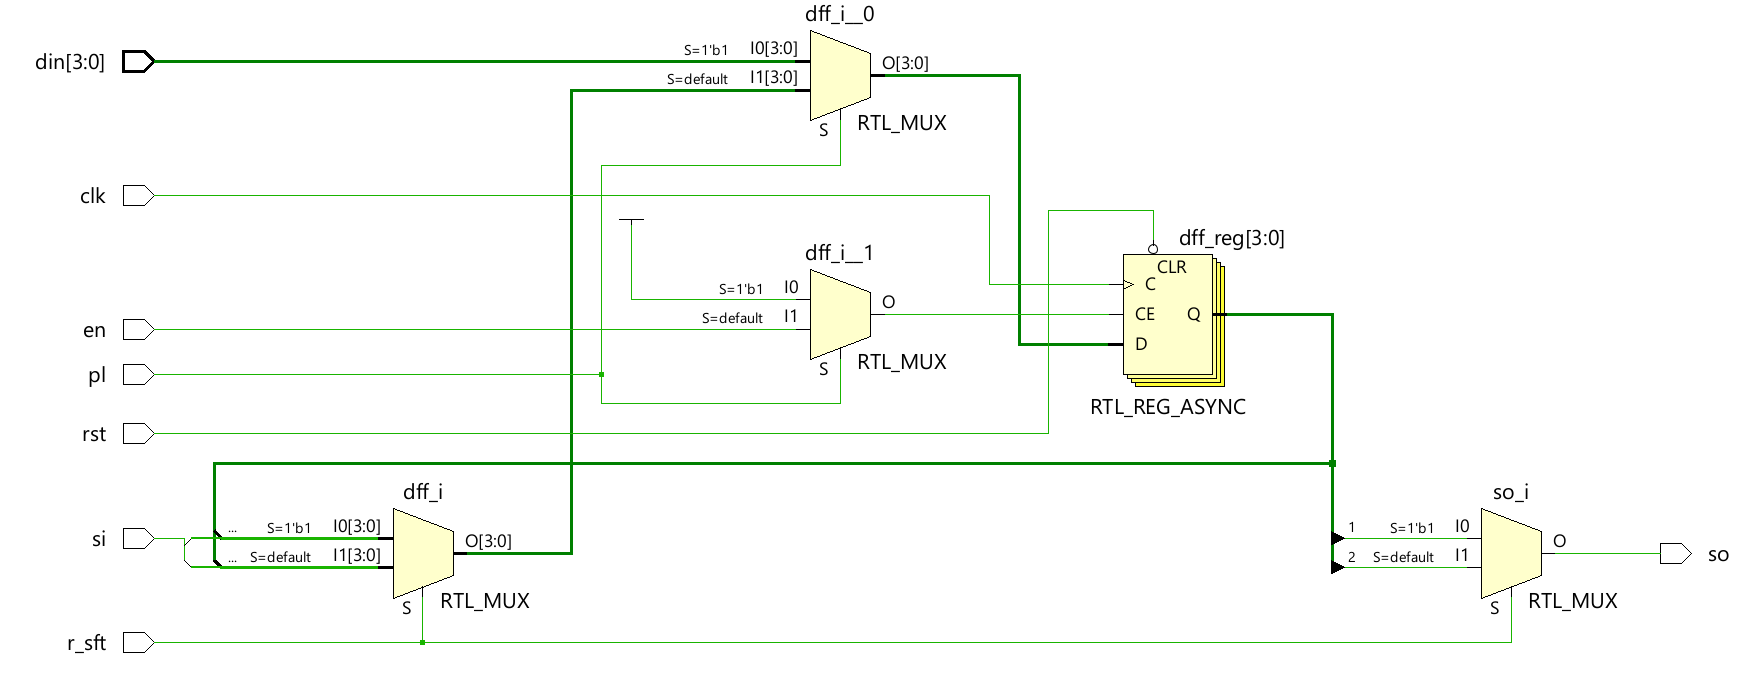
\includegraphics[width=0.9\textwidth]{RTL/shift_register.png}
    \caption{RTL σχηματικό του Shift Register}
    \label{fig:shift_register_rtl}
\end{figure}

Οι είσοδοι ελέγχου λειτουργούν με την ακόλουθη προτεραιότητα:
\begin{enumerate}
    \item \texttt{rst = '0'}: Ασύγχρονη επαναφορά (υψηλότερη προτεραιότητα)
    \item \texttt{pl = '1'}: Παράλληλη φόρτωση δεδομένων από \texttt{din}
    \item \texttt{en = '1'}: Ενεργοποίηση ολίσθησης
    \item \texttt{r\_sft}: Επιλογή κατεύθυνσης ολίσθησης (1=δεξιά, 0=αριστερά)
\end{enumerate}

Η σειριακή έξοδος \texttt{so} εξαρτάται από την κατεύθυνση ολίσθησης:
\begin{itemize}
    \item Shift Right: \texttt{so} = LSB (\texttt{dout(0)})
    \item Shift Left: \texttt{so} = MSB (\texttt{dout(3)})
\end{itemize}

\subsection*{Κώδικας VHDL}

\begin{lstlisting}[language=VHDL]
--------------------------------------------
-- 4 bit shift register with parallel load
--------------------------------------------

library IEEE;
use IEEE.std_logic_1164.all;
entity rl_shift_reg is
    port (
        clk,rst,si,en,pl,r_sft: in std_logic;
        din: in std_logic_vector(3 downto 0);
        dout: out std_logic_vector(3 downto 0);
        so: out std_logic
        );
end rl_shift_reg;

architecture rtl of rl_shift_reg is
    signal dff: std_logic_vector(3 downto 0);
begin
    edge: process (clk,rst)
    begin
        if rst='0' then
            dff<=(others=>'0');
        elsif rising_edge(clk) then
            if pl='1' then
                dff<=din;
            elsif en='1' then
                if r_sft = '1' then
                    dff<=si&dff(3 downto 1);
                else 
                    dff<=dff(2 downto 0)&si;
                end if;
            end if;
        end if;
    end process;
    so <= dff(0) when r_sft = '1' 
                 else dff(3);
    dout <= dff;
end rtl;
\end{lstlisting}

\subsection*{Testbench}

\begin{lstlisting}[language=VHDL]
---------------------------------------------------------------------
-- 4 bit register with parallel load and left/right shift testbench
---------------------------------------------------------------------

library IEEE;
use IEEE.STD_LOGIC_1164.ALL;
use IEEE.NUMERIC_STD.ALL;

entity rl_shift_reg_tb is
end entity;

architecture tb of rl_shift_reg_tb is
    component rl_shift_reg is 
        port (
        clk,rst,si,en,pl,r_sft: in std_logic;
        din: in std_logic_vector(3 downto 0);
        dout: out std_logic_vector(3 downto 0);
        so: out std_logic
        );
    end component;
    
    signal clk : std_logic;
    signal rst : std_logic;
    signal si : std_logic;
    signal en : std_logic;
    signal pl : std_logic;
    signal r_sft : std_logic;
    signal din : std_logic_vector(3 downto 0);
    signal dout : std_logic_vector(3 downto 0);
    signal so : std_logic;
    
    constant CLOCK_PERIOD : time := 10 ns;
    signal expected: std_logic_vector(3 downto 0);
    
begin
    DUT : rl_shift_reg
        port map (
            clk => clk,
            rst => rst,
            si => si,
            en => en,
            pl => pl,
            r_sft => r_sft,
            din => din,
            so => so,
            dout => dout
        );

    STIMULUS : process
    begin
        din <= (others => '0');
        si <= '0';
        en <= '0';
        pl <= '1';
        rst <= '1';
        r_sft <= '0';
        wait until falling_edge(clk);

        -- Test Parallel Load
        for i in 0 to 7 loop 
            din <= std_logic_vector(to_unsigned(i, 4));
            wait until falling_edge(clk);
            assert (din = dout)
                report "PARALLEL LOADING TEST FAILED! Mismatch at input index " & integer'image(i)
                severity error;
        end loop;
        assert false report "PARALLEL LOADING TEST FINISHED!" severity note;

        -- Test Shift Right
        pl <= '1';
        din <= (others => '0');
        wait until falling_edge(clk);

        pl <= '0';
        en <= '1';
        r_sft <= '1';
        si <= '1';
        expected <= (others => '0');
        
        wait for CLOCK_PERIOD * 5;
        assert false report "SHIFT RIGHT TEST FINISHED!" severity note;

        -- Test Shift Left
        pl <= '1';
        din <= (others => '0');
        wait until falling_edge(clk);

        r_sft <= '0';
        si <= '1';
        
        wait for CLOCK_PERIOD * 5;
        assert false report "SHIFT LEFT TEST FINISHED!" severity note;

        wait;
    end process;

    clk_gen : process
    begin
        clk <= '0';
        wait for CLOCK_PERIOD/2;
        clk <= '1';
        wait for CLOCK_PERIOD/2;
    end process;
end tb;
\end{lstlisting}

\subsection*{Ανάλυση Αποτελεσμάτων Testbench}

Το testbench ελέγχει τις ακόλουθες λειτουργίες:

\begin{enumerate}
    \item \textbf{Parallel Load}: Φόρτωση τιμών 0-7 στους καταχωρητές
    \item \textbf{Shift Right με '1'}: Ολίσθηση δεξιά με είσοδο '1' (εμφάνιση σειριακής εξόδου LSB)
    \item \textbf{Shift Right με '0'}: Ολίσθηση δεξιά με είσοδο '0'
    \item \textbf{Shift Left με '1'}: Ολίσθηση αριστερά με είσοδο '1' (εμφάνιση σειριακής εξόδου MSB)
    \item \textbf{Shift Left με '0'}: Ολίσθηση αριστερά με είσοδο '0'
    \item \textbf{Συνδυαστική λειτουργία}: Εναλλαγή μεταξύ parallel load και shift
\end{enumerate}

Η προσομοίωση επιβεβαίωσε την ορθή λειτουργία όλων των λειτουργιών του shift register.

% ==============================================================================
% ΜΕΡΟΣ Β
% ==============================================================================
\newpage
\section*{Μέρος Β}
\addcontentsline{toc}{section}{Μέρος Β}

% ------------------------------------------------------------------------------
% Β.1 Half Adder
% ------------------------------------------------------------------------------
\section*{Β.1 Ημιαθροιστής (Half Adder)}
\addcontentsline{toc}{subsection}{Β.1 Ημιαθροιστής (Half Adder)}

\subsection*{Περιγραφή Κυκλώματος}

Ο Ημιαθροιστής (Half Adder) είναι ένα συνδυαστικό κύκλωμα που εκτελεί πρόσθεση δύο bits. Αποτελεί τη βασική δομική μονάδα πάνω στην οποία θα χτιστούν τα υπόλοιπα κυκλώματα ιεραρχικά. Υλοποιήθηκε σε περιγραφή ροής δεδομένων (Dataflow).

Είσοδοι:
\begin{itemize}
    \item \texttt{i\_A}: Πρώτο bit εισόδου
    \item \texttt{i\_B}: Δεύτερο bit εισόδου
\end{itemize}

Έξοδοι:
\begin{itemize}
    \item \texttt{o\_Sum}: Άθροισμα ($S = A \oplus B$)
    \item \texttt{o\_Carry}: Κρατούμενο ($C = A \cdot B$)
\end{itemize}

\subsection*{Σχεδιάγραμμα Λειτουργίας}

\begin{figure}[H]
    \centering
    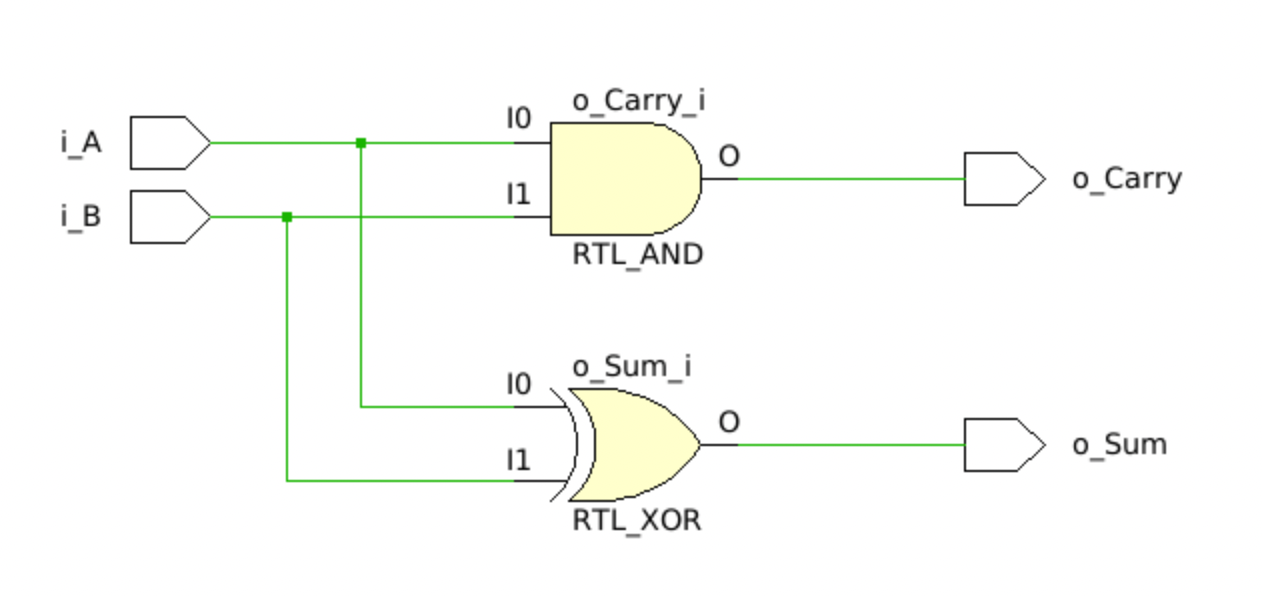
\includegraphics[width=0.5\textwidth]{RTL/half_adder.png}
    \caption{RTL σχηματικό του Half Adder}
    \label{fig:half_adder_rtl}
\end{figure}

Ο πίνακας αλήθειας του Half Adder:

\begin{table}[H]
    \centering
    \begin{tabular}{|c|c|c|c|}
        \hline
        \textbf{i\_A} & \textbf{i\_B} & \textbf{o\_Sum} & \textbf{o\_Carry} \\
        \hline
        0 & 0 & 0 & 0 \\
        \hline
        0 & 1 & 1 & 0 \\
        \hline
        1 & 0 & 1 & 0 \\
        \hline
        1 & 1 & 0 & 1 \\
        \hline
    \end{tabular}
    \caption{Πίνακας αλήθειας Half Adder}
    \label{tab:half_adder_truth}
\end{table}

\subsection*{Κώδικας VHDL - Dataflow Model}

\begin{lstlisting}[language=VHDL]
-------------------------------------------------------------------
-- Half Adder
-------------------------------------------------------------------

library ieee;
use ieee.std_logic_1164.all;
use ieee.numeric_std.all;

entity half_adder is
    Port (
        i_A : in STD_LOGIC;
        i_B : in STD_LOGIC;
        o_Sum : out STD_LOGIC;
        o_Carry : out STD_LOGIC
    );
end entity;

architecture Dataflow of half_adder is

begin

    o_Sum <= i_A XOR i_B;
    o_Carry <= i_A AND i_B;

end Dataflow;
\end{lstlisting}

\subsection*{Testbench}

\begin{lstlisting}[language=VHDL]
-------------------------------------------------------------------
-- Half Adder - Testbench
-------------------------------------------------------------------

library ieee;
use ieee.std_logic_1164.all;
use ieee.numeric_std.all;

entity half_adder_tb is
end entity;

architecture tb of half_adder_tb is
    component half_adder is
        port (
            i_A     : in    std_logic;
            i_B     : in    std_logic;
            o_Sum   : out   std_logic;
            o_Carry : out   std_logic
        );
    end component;

    signal i_A      : std_logic := '0';
    signal i_B      : std_logic := '0';
    signal o_Sum    : std_logic;
    signal o_Carry  : std_logic;

    constant TIME_DELAY : time := 10 ns;

begin

    DUT : half_adder
        port map (
            i_A     => i_A,
            i_B     => i_B,
            o_Sum   => o_Sum,
            o_Carry => o_Carry
        );

    STIMULUS : process
    begin
        i_A <= '0';
        i_B <= '0';
        wait for (1 * TIME_DELAY);

        i_A <= '0';
        i_B <= '0';
        wait for (1 * TIME_DELAY);
        assert (o_Sum = '0' and o_Carry = '0')
            report "FAIL: 0+0 expected Sum=0, Carry=0";

        i_A <= '0';
        i_B <= '1';
        wait for (1 * TIME_DELAY);
        assert (o_Sum = '1' and o_Carry = '0')
            report "FAIL: 0+1 expected Sum=1, Carry=0";

        i_A <= '1';
        i_B <= '0';
        wait for (1 * TIME_DELAY);
        assert (o_Sum = '1' and o_Carry = '0')
            report "FAIL: 1+0 expected Sum=1, Carry=0";

        i_A <= '1';
        i_B <= '1';
        wait for (1 * TIME_DELAY);
        assert (o_Sum = '0' and o_Carry = '1')
            report "FAIL: 1+1 expected Sum=0, Carry=1";

        wait;

    end process;
end architecture;
\end{lstlisting}

\subsection*{Ανάλυση Αποτελεσμάτων Testbench}

Το testbench ελέγχει εξαντλητικά όλους τους 4 δυνατούς συνδυασμούς εισόδου. Για κάθε συνδυασμό, επαληθεύεται ότι τόσο το άθροισμα όσο και το κρατούμενο αντιστοιχούν στις αναμενόμενες τιμές σύμφωνα με τον πίνακα αλήθειας. Εφόσον δεν υπήρχε κάποιο assert error κατά την εκτέλεση της προσομοίωσης, επιβεβαιώθηκε η ορθή λειτουργία του κυκλώματος.

\subsection*{Κρίσιμο Μονοπάτι (Critical Path)}

\begin{figure}[H]
    \centering
    
\includegraphics[width=0.9\textwidth]{critical_paths/half_adder.png}
    \caption{Κρίσιμο μονοπάτι του Half Adder}
    \label{fig:half_adder_critical}
\end{figure}

Το κρίσιμο μονοπάτι του Half Adder είναι από την είσοδο \texttt{i\_B} προς την έξοδο \texttt{o\_Sum} με συνολική καθυστέρηση \textbf{5.377 ns} (Logic Delay: 3.778 ns, Net Delay: 1.599 ns). Το μονοπάτι διέρχεται από 3 επίπεδα λογικής (levels) και 4 routes.

% ------------------------------------------------------------------------------
% Β.2 Full Adder
% ------------------------------------------------------------------------------
\newpage
\section*{Β.2 Πλήρης Αθροιστής (Full Adder)}
\addcontentsline{toc}{subsection}{Β.2 Πλήρης Αθροιστής (Full Adder)}

\subsection*{Περιγραφή Κυκλώματος}

Ο Πλήρης Αθροιστής (Full Adder) εκτελεί πρόσθεση τριών bits (δύο bits εισόδου και ένα κρατούμενο εισόδου). Υλοποιήθηκε με δομική περιγραφή (Structural), χρησιμοποιώντας δύο instances του Half Adder και μία πύλη OR για τον υπολογισμό του τελικού κρατούμενου εξόδου.

Είσοδοι:
\begin{itemize}
    \item \texttt{i\_A}: Πρώτο bit εισόδου
    \item \texttt{i\_B}: Δεύτερο bit εισόδου
    \item \texttt{i\_Carry\_in}: Κρατούμενο εισόδου
\end{itemize}

Έξοδοι:
\begin{itemize}
    \item \texttt{o\_Sum}: Άθροισμα
    \item \texttt{o\_Carry\_out}: Κρατούμενο εξόδου
\end{itemize}

\subsection*{Σχεδιάγραμμα Λειτουργίας}

\begin{figure}[H]
    \centering
    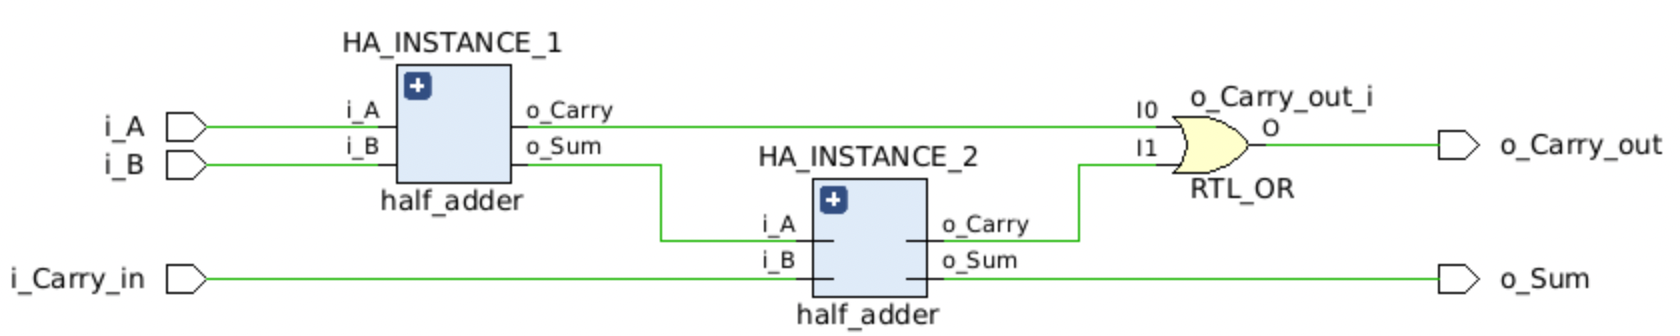
\includegraphics[width=0.7\textwidth]{RTL/full_adder.png}
    \caption{RTL σχηματικό του Full Adder}
    \label{fig:full_adder_rtl}
\end{figure}

Ο πίνακας αλήθειας του Full Adder:

\begin{table}[H]
    \centering
    \begin{tabular}{|c|c|c|c|c|}
        \hline
        \textbf{i\_A} & \textbf{i\_B} & \textbf{i\_Carry\_in} & \textbf{o\_Sum} & \textbf{o\_Carry\_out} \\
        \hline
        0 & 0 & 0 & 0 & 0 \\
        \hline
        0 & 0 & 1 & 1 & 0 \\
        \hline
        0 & 1 & 0 & 1 & 0 \\
        \hline
        0 & 1 & 1 & 0 & 1 \\
        \hline
        1 & 0 & 0 & 1 & 0 \\
        \hline
        1 & 0 & 1 & 0 & 1 \\
        \hline
        1 & 1 & 0 & 0 & 1 \\
        \hline
        1 & 1 & 1 & 1 & 1 \\
        \hline
    \end{tabular}
    \caption{Πίνακας αλήθειας Full Adder}
    \label{tab:full_adder_truth}
\end{table}

Η δομή του κυκλώματος βασίζεται στην αποσύνθεση του Full Adder σε δύο Half Adders: ο πρώτος υπολογίζει $A \oplus B$ και $A \cdot B$, ενώ ο δεύτερος υπολογίζει $(A \oplus B) \oplus C_{in}$ και $(A \oplus B) \cdot C_{in}$. Το τελικό κρατούμενο εξόδου προκύπτει ως $C_{out} = (A \cdot B) + ((A \oplus B) \cdot C_{in})$.

\subsection*{Κώδικας VHDL - Structural Model}

\begin{lstlisting}[language=VHDL]
library IEEE;
use IEEE.STD_LOGIC_1164.ALL;

entity full_adder is
    Port (
        i_A : in STD_LOGIC;
        i_B : in STD_LOGIC;
        i_Carry_in : in STD_LOGIC;
        o_Sum : out STD_LOGIC;
        o_Carry_out : out STD_LOGIC
    );
end entity;

architecture Structural of full_adder is

    component half_adder is
        Port (
            i_A : in STD_LOGIC;
            i_B : in STD_LOGIC;
            o_Sum : out STD_LOGIC;
            o_Carry : out STD_LOGIC
        );
    end component;

    signal sum_1, carry_1, carry_2 : std_logic := '0';

begin

    HA_INSTANCE_1 : half_adder
        port map (
            i_A => i_A,
            i_B => i_B,
            o_Sum => sum_1,
            o_Carry => carry_1
        );

    HA_INSTANCE_2 : half_adder
        port map (
            i_A => sum_1,
            i_B => i_Carry_in,
            o_Sum => o_Sum,
            o_Carry => carry_2
        );

    o_Carry_out <= carry_1 OR carry_2;

end Structural;
\end{lstlisting}

\subsection*{Testbench}

\begin{lstlisting}[language=VHDL]
library IEEE;
use IEEE.STD_LOGIC_1164.ALL;

entity full_adder_tb is
end entity;

architecture tb of full_adder_tb is

    component full_adder is
        Port (
            i_A : in STD_LOGIC;
            i_B : in STD_LOGIC;
            i_Carry_in : in STD_LOGIC;
            o_Sum : out STD_LOGIC;
            o_Carry_out : out STD_LOGIC
        );
    end component;

    signal i_A, i_B, i_Carry_in : std_logic := '0';
    signal o_Sum, o_Carry_out : std_logic;

    constant TIME_DELAY : time := 10 ns;

begin

    DUT: full_adder
        port map (
            i_A => i_A,
            i_B => i_B,
            i_Carry_in => i_Carry_in,
            o_Sum => o_Sum,
            o_Carry_out => o_Carry_out
        );

    STIMULUS: process
    begin
        i_A <= '0'; i_B <= '0'; i_Carry_in <= '0';
        wait for (1 * TIME_DELAY);
        assert (o_Sum = '0' and o_Carry_out = '0')
            report "FAIL: 0+0+0 expected Sum=0, Carry=0";

        i_A <= '0'; i_B <= '0'; i_Carry_in <= '1';
        wait for (1 * TIME_DELAY);
        assert (o_Sum = '1' and o_Carry_out = '0')
            report "FAIL: 0+0+1 expected Sum=1, Carry=0";

        i_A <= '0'; i_B <= '1'; i_Carry_in <= '0';
        wait for (1 * TIME_DELAY);
        assert (o_Sum = '1' and o_Carry_out = '0')
            report "FAIL: 0+1+0 expected Sum=1, Carry=0";

        i_A <= '0'; i_B <= '1'; i_Carry_in <= '1';
        wait for (1 * TIME_DELAY);
        assert (o_Sum = '0' and o_Carry_out = '1')
            report "FAIL: 0+1+1 expected Sum=0, Carry=1";

        i_A <= '1'; i_B <= '0'; i_Carry_in <= '0';
        wait for (1 * TIME_DELAY);
        assert (o_Sum = '1' and o_Carry_out = '0')
            report "FAIL: 1+0+0 expected Sum=1, Carry=0";

        i_A <= '1'; i_B <= '0'; i_Carry_in <= '1';
        wait for (1 * TIME_DELAY);
        assert (o_Sum = '0' and o_Carry_out = '1')
            report "FAIL: 1+0+1 expected Sum=0, Carry=1";

        i_A <= '1'; i_B <= '1'; i_Carry_in <= '0';
        wait for (1 * TIME_DELAY);
        assert (o_Sum = '0' and o_Carry_out = '1')
            report "FAIL: 1+1+0 expected Sum=0, Carry=1";

        i_A <= '1'; i_B <= '1'; i_Carry_in <= '1';
        wait for (1 * TIME_DELAY);
        assert (o_Sum = '1' and o_Carry_out = '1')
            report "FAIL: 1+1+1 expected Sum=1, Carry=1";

        report "All tests passed!";
        wait;
    end process;

end architecture tb;
\end{lstlisting}

\subsection*{Ανάλυση Αποτελεσμάτων Testbench}

Το testbench ελέγχει εξαντλητικά όλους τους 8 δυνατούς συνδυασμούς εισόδου ($2^3 = 8$). Για κάθε συνδυασμό, επαληθεύεται ότι τόσο το άθροισμα όσο και το κρατούμενο εξόδου αντιστοιχούν στις αναμενόμενες τιμές. Εφόσον δεν υπήρχε κάποιο assert error κατά την εκτέλεση της προσομοίωσης, επιβεβαιώθηκε η ορθή λειτουργία του κυκλώματος.

\subsection*{Κρίσιμο Μονοπάτι (Critical Path)}

\begin{figure}[H]
    \centering
    
\includegraphics[width=0.9\textwidth]{critical_paths/full_adder.png}
    \caption{Κρίσιμο μονοπάτι του Full Adder}
    \label{fig:full_adder_critical}
\end{figure}

Το κρίσιμο μονοπάτι του Full Adder είναι από την είσοδο \texttt{i\_A} προς την έξοδο \texttt{o\_Sum} με συνολική καθυστέρηση \textbf{5.377 ns} (Logic Delay: 3.778 ns, Net Delay: 1.599 ns). Το μονοπάτι διέρχεται από 3 επίπεδα λογικής και 4 routes. Παρατηρούμε ότι η καθυστέρηση είναι ίδια με αυτή του Half Adder, καθώς το Vivado βελτιστοποιεί τη δομική ιεραρχία κατά τη σύνθεση.

% ------------------------------------------------------------------------------
% Β.3 4-bit Parallel Adder
% ------------------------------------------------------------------------------
\newpage
\section*{Β.3 Παράλληλος Αθροιστής 4 bits (4-bit Parallel Adder)}
\addcontentsline{toc}{subsection}{Β.3 Παράλληλος Αθροιστής 4 bits}

\subsection*{Περιγραφή Κυκλώματος}

Ο Παράλληλος Αθροιστής 4 bits (4-bit Parallel Adder) εκτελεί πρόσθεση δύο 4-bit αριθμών με κρατούμενο εισόδου. Υλοποιήθηκε με δομική περιγραφή (Structural) χρησιμοποιώντας τέσσερα instances του Full Adder συνδεδεμένα σε αλυσίδα (ripple carry), όπου το κρατούμενο εξόδου κάθε βαθμίδας τροφοδοτεί το κρατούμενο εισόδου της επόμενης.

Είσοδοι:
\begin{itemize}
    \item \texttt{i\_A(3:0)}: Πρώτος 4-bit αριθμός
    \item \texttt{i\_B(3:0)}: Δεύτερος 4-bit αριθμός
    \item \texttt{i\_Carry\_in}: Κρατούμενο εισόδου
\end{itemize}

Έξοδοι:
\begin{itemize}
    \item \texttt{o\_Sum(3:0)}: 4-bit άθροισμα
    \item \texttt{o\_Carry\_out}: Κρατούμενο εξόδου
\end{itemize}

\subsection*{Σχεδιάγραμμα Λειτουργίας}

\begin{figure}[H]
    \centering
    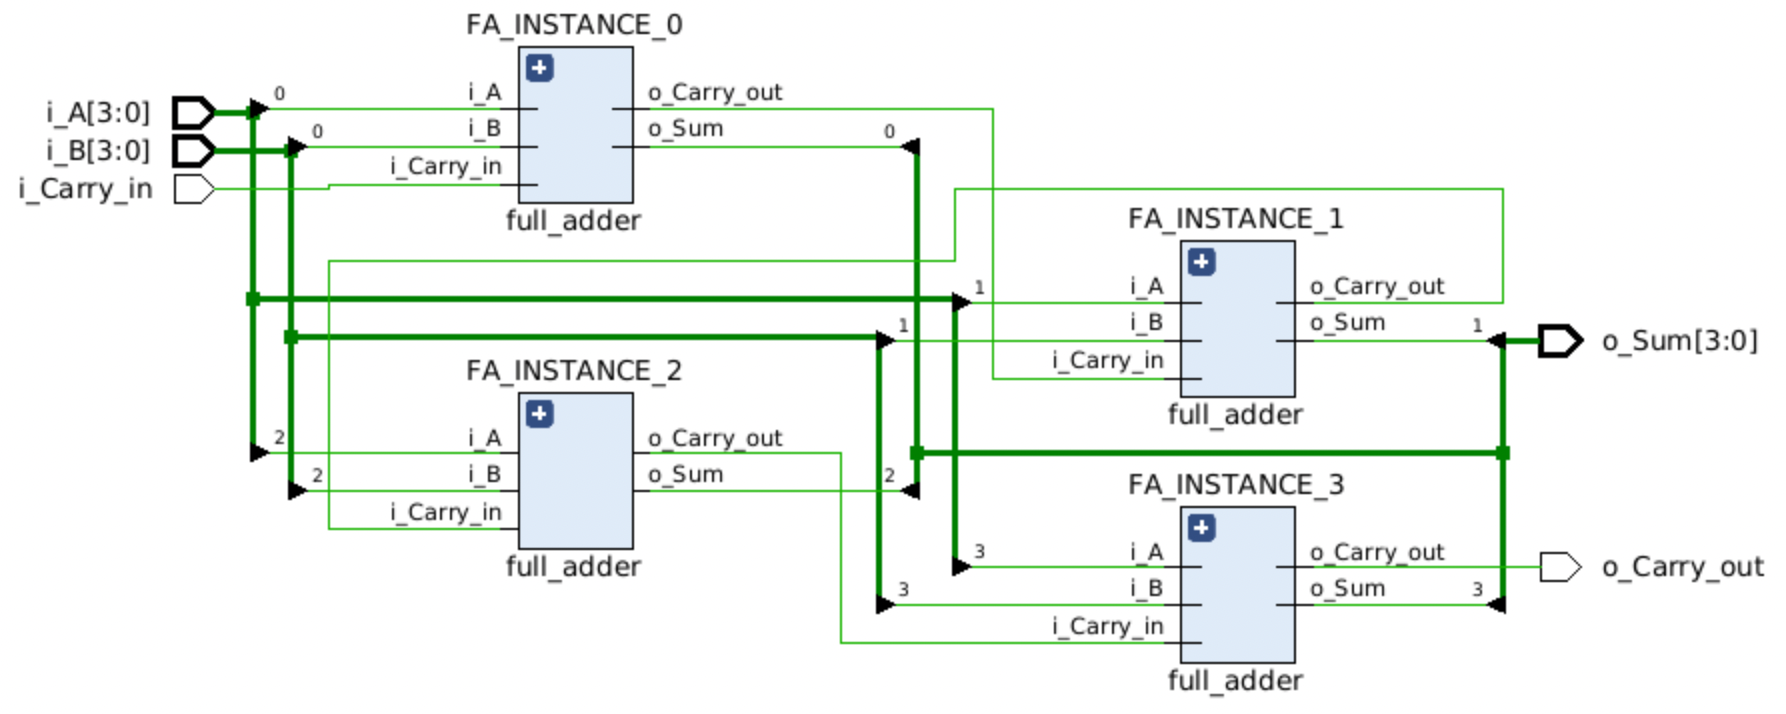
\includegraphics[width=0.9\textwidth]{RTL/4bit_parallel_adder.png}
    \caption{RTL σχηματικό του 4-bit Parallel Adder}
    \label{fig:4bit_pa_rtl}
\end{figure}

Η αρχιτεκτονική ripple carry αποτελείται από τέσσερις Full Adders σε σειρά. Κάθε Full Adder υπολογίζει ένα bit του αθροίσματος και παράγει ένα κρατούμενο που μεταφέρεται στον επόμενο Full Adder. Το σήμα \texttt{carry} χρησιμοποιείται ως εσωτερικό σήμα 5 bits για τη διασύνδεση των κρατούμενων.

\subsection*{Κώδικας VHDL - Structural Model}

\begin{lstlisting}[language=VHDL]
library IEEE;
use IEEE.STD_LOGIC_1164.ALL;

entity parallel_adder_4bit is
    Port (
        i_A : in  STD_LOGIC_VECTOR(3 downto 0);
        i_B : in  STD_LOGIC_VECTOR(3 downto 0);
        i_Carry_in : in  STD_LOGIC;
        o_Sum : out STD_LOGIC_VECTOR(3 downto 0);
        o_Carry_out : out STD_LOGIC
    );
end entity;

architecture Structural of parallel_adder_4bit is

    component full_adder is
        Port (
        i_A : in STD_LOGIC;
        i_B : in STD_LOGIC;
        i_Carry_in : in STD_LOGIC;
        o_Sum : out STD_LOGIC;
        o_Carry_out : out STD_LOGIC
    );
    end component;

    signal carry : std_logic_vector(4 downto 0) := (others => '0');

begin

    FA_INSTANCE_0 : full_adder
        port map (
            i_A => i_A(0),
            i_B => i_B(0),
            i_Carry_in => carry(0),
            o_Sum => o_Sum(0),
            o_Carry_out => carry(1)
        );

    FA_INSTANCE_1 : full_adder
        port map (
            i_A => i_A(1),
            i_B => i_B(1),
            i_Carry_in => carry(1),
            o_Sum => o_Sum(1),
            o_Carry_out => carry(2)
        );

    FA_INSTANCE_2 : full_adder
        port map (
            i_A => i_A(2),
            i_B => i_B(2),
            i_Carry_in => carry(2),
            o_Sum => o_Sum(2),
            o_Carry_out => carry(3)
        );

    FA_INSTANCE_3 : full_adder
        port map (
            i_A => i_A(3),
            i_B => i_B(3),
            i_Carry_in => carry(3),
            o_Sum => o_Sum(3),
            o_Carry_out => carry(4)
        );

    carry(0) <= i_Carry_in;
    o_Carry_out <= carry(4);

end Structural;
\end{lstlisting}

\subsection*{Testbench}

\begin{lstlisting}[language=VHDL]
library IEEE;
use IEEE.STD_LOGIC_1164.ALL;
use IEEE.NUMERIC_STD.ALL;

entity parallel_adder_4bit_tb is
end entity;

architecture tb of parallel_adder_4bit_tb is

    component parallel_adder_4bit is
        Port (
            i_A : in  STD_LOGIC_VECTOR(3 downto 0);
            i_B : in  STD_LOGIC_VECTOR(3 downto 0);
            i_Carry_in : in  STD_LOGIC;
            o_Sum : out STD_LOGIC_VECTOR(3 downto 0);
            o_Carry_out : out STD_LOGIC
        );
    end component;

    signal i_A, i_B : std_logic_vector(3 downto 0) := (others => '0');
    signal i_Carry_in : std_logic := '0';
    signal o_Sum : std_logic_vector(3 downto 0);
    signal o_Carry_out : std_logic;

    constant TIME_DELAY : time := 10 ns;

begin

    DUT: parallel_adder_4bit
        port map (
            i_A => i_A,
            i_B => i_B,
            i_Carry_in => i_Carry_in,
            o_Sum => o_Sum,
            o_Carry_out => o_Carry_out
        );

    STIMULUS: process
        variable expected_sum   : integer;
        variable expected_carry : std_logic;
        variable total          : integer;
    begin
        for a in 0 to 15 loop
            for b in 0 to 15 loop
                for cin in 0 to 1 loop
                    i_A        <= std_logic_vector(to_unsigned(a, 4));
                    i_B        <= std_logic_vector(to_unsigned(b, 4));
                    i_Carry_in <= std_logic(to_unsigned(cin, 1)(0));
                    wait for TIME_DELAY;

                    total        := a + b + cin;
                    expected_sum := total mod 16;

                    if total > 15 then
                        expected_carry := '1';
                    else
                        expected_carry := '0';
                    end if;

                    assert (o_Sum = std_logic_vector(
                                to_unsigned(expected_sum, 4))
                            and o_Carry_out = expected_carry)
                        report "FAIL: " & integer'image(a) & "+"
                               & integer'image(b) & "+"
                               & integer'image(cin)
                        severity failure;
                end loop;
            end loop;
        end loop;
        report "All 512 test cases passed!" severity note;
        wait;
    end process;

end architecture tb;
\end{lstlisting}

\subsection*{Ανάλυση Αποτελεσμάτων Testbench}

Το testbench ελέγχει εξαντλητικά όλους τους $16 \times 16 \times 2 = 512$ δυνατούς συνδυασμούς εισόδου. Για κάθε συνδυασμό υπολογίζεται το αναμενόμενο άθροισμα και κρατούμενο, και συγκρίνεται με τις εξόδους του κυκλώματος. Εφόσον δεν υπήρχε κάποιο assert error κατά την εκτέλεση, επιβεβαιώθηκε η ορθή λειτουργία του 4-bit Parallel Adder για όλες τις δυνατές εισόδους.

\subsection*{Κρίσιμο Μονοπάτι (Critical Path)}

\begin{figure}[H]
    \centering
    
\includegraphics[width=0.9\textwidth]{critical_paths/4bit_parallel_adder.png}
    \caption{Κρίσιμο μονοπάτι του 4-bit Parallel Adder}
    \label{fig:4bit_pa_critical}
\end{figure}

Το κρίσιμο μονοπάτι του 4-bit Parallel Adder είναι από την είσοδο \texttt{i\_B[0]} προς τις εξόδους \texttt{o\_Carry\_out} και \texttt{o\_Sum[2]} με συνολική καθυστέρηση \textbf{5.970 ns} (Logic Delay: 3.904 ns, Net Delay: 2.066 ns). Το μονοπάτι διέρχεται από 4 επίπεδα λογικής και 5 routes. Η αυξημένη καθυστέρηση σε σχέση με τον Full Adder οφείλεται στη διάδοση του κρατούμενου (ripple carry) μέσω των διαδοχικών βαθμίδων.

% ------------------------------------------------------------------------------
% Β.4 BCD Full Adder
% ------------------------------------------------------------------------------
\newpage
\section*{Β.4 BCD Πλήρης Αθροιστής (BCD Full Adder)}
\addcontentsline{toc}{subsection}{Β.4 BCD Πλήρης Αθροιστής (BCD Full Adder)}

\subsection*{Περιγραφή Κυκλώματος}

Ο BCD Πλήρης Αθροιστής εκτελεί πρόσθεση δύο BCD ψηφίων (0-9) με κρατούμενο εισόδου. Υλοποιήθηκε με δομική περιγραφή (Structural) χρησιμοποιώντας δύο instances του 4-bit Parallel Adder και επιπλέον συνδυαστική λογική για τη διόρθωση BCD.

Η λογική λειτουργίας είναι η εξής:
\begin{enumerate}
    \item Πρώτα εκτελείται κανονική δυαδική πρόσθεση των δύο BCD ψηφίων μέσω του πρώτου 4-bit PA
    \item Ελέγχεται αν το αποτέλεσμα υπερβαίνει το 9 (δηλαδή αν υπάρχει κρατούμενο ή αν $S_3 \cdot S_2 + S_3 \cdot S_1 = 1$)
    \item Αν απαιτείται διόρθωση, προστίθεται η τιμή 6 (0110) μέσω του δεύτερου 4-bit PA
\end{enumerate}

Είσοδοι:
\begin{itemize}
    \item \texttt{i\_A(3:0)}: Πρώτο BCD ψηφίο (0-9)
    \item \texttt{i\_B(3:0)}: Δεύτερο BCD ψηφίο (0-9)
    \item \texttt{i\_Carry\_in}: Κρατούμενο εισόδου
\end{itemize}

Έξοδοι:
\begin{itemize}
    \item \texttt{o\_Sum(3:0)}: BCD ψηφίο αθροίσματος (0-9)
    \item \texttt{o\_Carry\_out}: Κρατούμενο εξόδου
\end{itemize}

\subsection*{Σχεδιάγραμμα Λειτουργίας}

\begin{figure}[H]
    \centering
    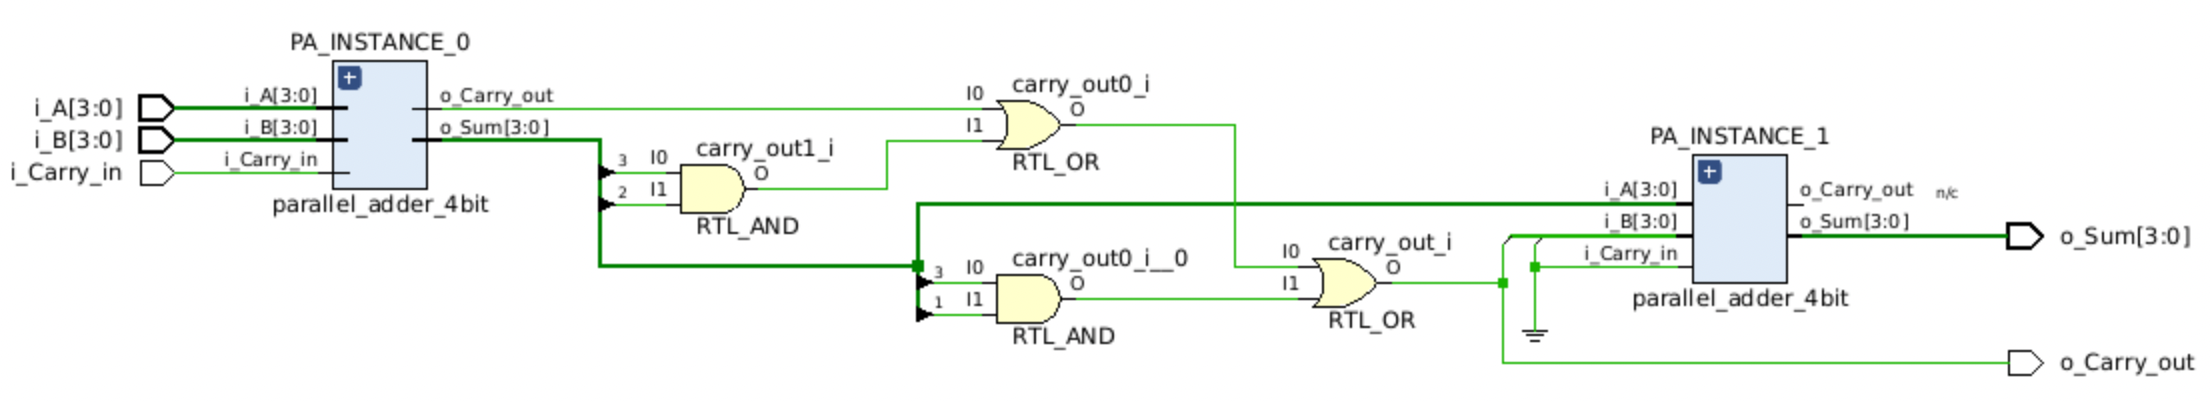
\includegraphics[width=0.9\textwidth]{RTL/bcd_full_adder.png}
    \caption{RTL σχηματικό του BCD Full Adder}
    \label{fig:bcd_fa_rtl}
\end{figure}

Η συνθήκη διόρθωσης υπολογίζεται ως:
$$C_{out} = C_1 + (S_3 \cdot S_2) + (S_3 \cdot S_1)$$

όπου $C_1$ είναι το κρατούμενο από την πρώτη πρόσθεση και $S_3, S_2, S_1$ τα bits του ενδιάμεσου αθροίσματος. Όταν $C_{out} = 1$, το σήμα διόρθωσης \texttt{correction} γίνεται ``0110'' (6), αλλιώς παραμένει ``0000''.

\subsection*{Κώδικας VHDL - Structural Model}

\begin{lstlisting}[language=VHDL]
library IEEE;
use IEEE.STD_LOGIC_1164.ALL;

entity bcd_full_adder is
    Port (
        i_A : in STD_LOGIC_VECTOR (3 downto 0);
        i_B : in STD_LOGIC_VECTOR (3 downto 0);
        i_Carry_in : in STD_LOGIC;
        o_Sum : out STD_LOGIC_VECTOR (3 downto 0);
        o_Carry_out : out STD_LOGIC
    );
end bcd_full_adder;

architecture Structural of bcd_full_adder is

    component parallel_adder_4bit is
        Port (
        i_A : in  STD_LOGIC_VECTOR(3 downto 0);
        i_B : in  STD_LOGIC_VECTOR(3 downto 0);
        i_Carry_in : in  STD_LOGIC;
        o_Sum : out STD_LOGIC_VECTOR(3 downto 0);
        o_Carry_out : out STD_LOGIC
    );
    end component;

    signal raw_sum : std_logic_vector(3 downto 0);
    signal carry_1 : std_logic;
    signal correction : std_logic_vector(3 downto 0);
    signal carry_out : std_logic;
    signal carry_2 : std_logic;

begin

    PA_INSTANCE_0 : parallel_adder_4bit
        port map (
            i_A => i_A,
            i_B => i_B,
            i_Carry_in => i_Carry_in,
            o_Sum => raw_sum,
            o_Carry_out => carry_1
        );

    carry_out <= carry_1 OR
                 (raw_sum(3) AND raw_sum(2)) OR
                 (raw_sum(3) AND raw_sum(1));

    correction(3) <= '0';
    correction(2) <= carry_out;
    correction(1) <= carry_out;
    correction(0) <= '0';

    PA_INSTANCE_1 : parallel_adder_4bit
        port map (
            i_A => raw_sum,
            i_B => correction,
            i_Carry_in => '0',
            o_Sum => o_Sum,
            o_Carry_out => carry_2
        );

    o_Carry_out <= carry_out;
end Structural;
\end{lstlisting}

\subsection*{Testbench}

\begin{lstlisting}[language=VHDL]
library IEEE;
use IEEE.STD_LOGIC_1164.ALL;
use IEEE.NUMERIC_STD.ALL;

entity bcd_full_adder_tb is
end entity;

architecture tb of bcd_full_adder_tb is

    component bcd_full_adder is
        Port (
            i_A         : in  STD_LOGIC_VECTOR(3 downto 0);
            i_B         : in  STD_LOGIC_VECTOR(3 downto 0);
            i_Carry_in  : in  STD_LOGIC;
            o_Sum       : out STD_LOGIC_VECTOR(3 downto 0);
            o_Carry_out : out STD_LOGIC
        );
    end component;

    signal i_A         : STD_LOGIC_VECTOR(3 downto 0) := (others => '0');
    signal i_B         : STD_LOGIC_VECTOR(3 downto 0) := (others => '0');
    signal i_Carry_in  : STD_LOGIC := '0';
    signal o_Sum       : STD_LOGIC_VECTOR(3 downto 0);
    signal o_Carry_out : STD_LOGIC;

    constant TIME_DELAY : time := 10 ns;

begin

    DUT: bcd_full_adder
        port map (
            i_A         => i_A,
            i_B         => i_B,
            i_Carry_in  => i_Carry_in,
            o_Sum       => o_Sum,
            o_Carry_out => o_Carry_out
        );

    STIMULUS: process
        variable total          : integer;
        variable expected_sum   : integer;
        variable expected_carry : std_logic;
    begin
        for a in 0 to 9 loop
            for b in 0 to 9 loop
                for cin in 0 to 1 loop
                    i_A        <= std_logic_vector(to_unsigned(a, 4));
                    i_B        <= std_logic_vector(to_unsigned(b, 4));
                    i_Carry_in <= std_logic(
                                    to_unsigned(cin, 1)(0));
                    wait for TIME_DELAY;

                    total := a + b + cin;

                    if total > 9 then
                        expected_sum   := total - 10;
                        expected_carry := '1';
                    else
                        expected_sum   := total;
                        expected_carry := '0';
                    end if;

                    assert (o_Sum = std_logic_vector(
                                to_unsigned(expected_sum, 4))
                            and o_Carry_out = expected_carry)
                        report "FAIL: " & integer'image(a) & "+"
                               & integer'image(b) & "+"
                               & integer'image(cin)
                        severity failure;
                end loop;
            end loop;
        end loop;

        report "All BCD tests passed!" severity note;
        wait;
    end process;

end architecture tb;
\end{lstlisting}

\subsection*{Ανάλυση Αποτελεσμάτων Testbench}

Το testbench ελέγχει εξαντλητικά όλους τους $10 \times 10 \times 2 = 200$ έγκυρους συνδυασμούς BCD εισόδου (ψηφία 0-9 με κρατούμενο 0 ή 1). Για κάθε συνδυασμό, ελέγχεται ότι το αποτέλεσμα είναι σωστό BCD ψηφίο (0-9) και ότι το κρατούμενο εξόδου ενεργοποιείται σωστά όταν το άθροισμα υπερβαίνει το 9. Εφόσον δεν υπήρχε κάποιο assert error κατά την εκτέλεση, επιβεβαιώθηκε η ορθή λειτουργία του BCD Full Adder.

\subsection*{Κρίσιμο Μονοπάτι (Critical Path)}

\begin{figure}[H]
    \centering
    
\includegraphics[width=0.9\textwidth]{critical_paths/bcd_full_adder.png}
    \caption{Κρίσιμο μονοπάτι του BCD Full Adder}
    \label{fig:bcd_fa_critical}
\end{figure}

Το κρίσιμο μονοπάτι του BCD Full Adder είναι από την είσοδο \texttt{i\_B[0]} προς την έξοδο \texttt{o\_Sum[3]} με συνολική καθυστέρηση \textbf{5.976 ns} (Logic Delay: 3.904 ns, Net Delay: 2.072 ns). Το μονοπάτι διέρχεται από 4 επίπεδα λογικής και 5 routes. Η καθυστέρηση είναι ελαφρώς μεγαλύτερη από αυτή του 4-bit PA λόγω της επιπλέον λογικής διόρθωσης BCD και του δεύτερου αθροιστή.

% ------------------------------------------------------------------------------
% Β.5 4-BCD Parallel Adder
% ------------------------------------------------------------------------------
\newpage
\section*{Β.5 Παράλληλος BCD Αθροιστής 4 ψηφίων (4-BCD Parallel Adder)}
\addcontentsline{toc}{subsection}{Β.5 Παράλληλος BCD Αθροιστής 4 ψηφίων}

\subsection*{Περιγραφή Κυκλώματος}

Ο Παράλληλος BCD Αθροιστής 4 ψηφίων εκτελεί πρόσθεση δύο 4-ψήφιων BCD αριθμών (0000-9999). Υλοποιήθηκε με δομική περιγραφή (Structural) χρησιμοποιώντας τέσσερα instances του BCD Full Adder συνδεδεμένα σε αλυσίδα, όπου το κρατούμενο εξόδου κάθε ψηφίου τροφοδοτεί το κρατούμενο εισόδου του επόμενου.

Είσοδοι:
\begin{itemize}
    \item \texttt{i\_A(15:0)}: Πρώτος 4-ψήφιος BCD αριθμός (4 ψηφία × 4 bits)
    \item \texttt{i\_B(15:0)}: Δεύτερος 4-ψήφιος BCD αριθμός
    \item \texttt{i\_Carry\_in}: Κρατούμενο εισόδου
\end{itemize}

Έξοδοι:
\begin{itemize}
    \item \texttt{o\_Sum(15:0)}: 4-ψήφιο BCD άθροισμα
    \item \texttt{o\_Carry\_out}: Κρατούμενο εξόδου (υπερχείλιση πέρα από 9999)
\end{itemize}

\subsection*{Σχεδιάγραμμα Λειτουργίας}

\begin{figure}[H]
    \centering
    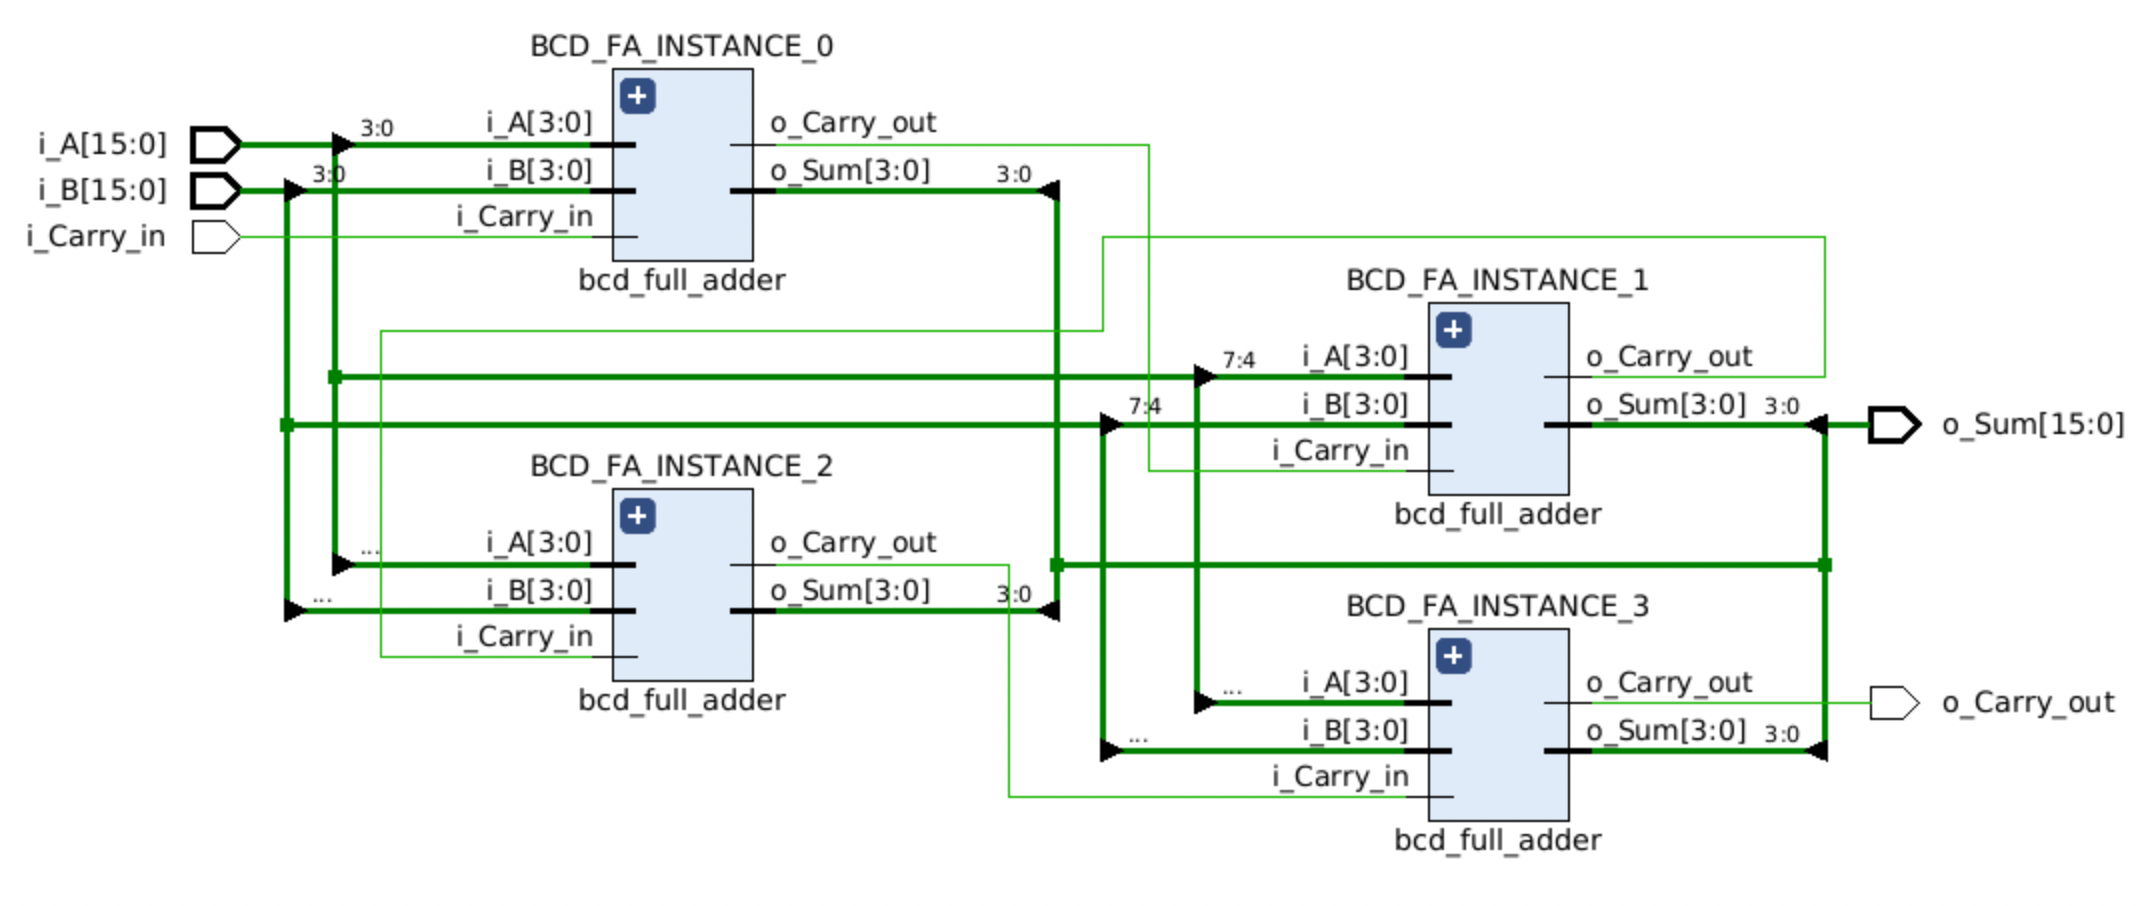
\includegraphics[width=0.9\textwidth]{RTL/bcd_parallel_adder_4bit.png}
    \caption{RTL σχηματικό του 4-BCD Parallel Adder}
    \label{fig:4bcd_pa_rtl}
\end{figure}

Η αρχιτεκτονική αποτελείται από τέσσερις BCD Full Adders σε σειρά. Κάθε BCD FA επεξεργάζεται ένα BCD ψηφίο (4 bits) και το κρατούμενο διαδίδεται μέσω του εσωτερικού σήματος \texttt{carry(2:0)} από το λιγότερο σημαντικό ψηφίο (bits 3:0) προς το πιο σημαντικό (bits 15:12).

\subsection*{Κώδικας VHDL - Structural Model}

\begin{lstlisting}[language=VHDL]
library IEEE;
use IEEE.STD_LOGIC_1164.ALL;

entity bcd_parallel_adder_4bit is
    Port (
        i_A : in STD_LOGIC_VECTOR (15 downto 0);
        i_B : in STD_LOGIC_VECTOR (15 downto 0);
        i_Carry_in : in STD_LOGIC;
        o_Sum : out STD_LOGIC_VECTOR (15 downto 0);
        o_Carry_out : out STD_LOGIC
    );
end bcd_parallel_adder_4bit;

architecture Structural of bcd_parallel_adder_4bit is

    component bcd_full_adder is
        Port (
        i_A : in STD_LOGIC_VECTOR (3 downto 0);
        i_B : in STD_LOGIC_VECTOR (3 downto 0);
        i_Carry_in : in STD_LOGIC;
        o_Sum : out STD_LOGIC_VECTOR (3 downto 0);
        o_Carry_out : out STD_LOGIC
    );
    end component;

    signal carry : std_logic_vector(2 downto 0) := (others => '0');

begin

    BCD_FA_INSTANCE_0 : bcd_full_adder
        port map (
            i_A => i_A(3 downto 0),
            i_B => i_B(3 downto 0),
            i_Carry_in => i_Carry_in,
            o_Sum => o_Sum(3 downto 0),
            o_Carry_out => carry(0)
        );

    BCD_FA_INSTANCE_1 : bcd_full_adder
        port map (
            i_A => i_A(7 downto 4),
            i_B => i_B(7 downto 4),
            i_Carry_in => carry(0),
            o_Sum => o_Sum(7 downto 4),
            o_Carry_out => carry(1)
        );

    BCD_FA_INSTANCE_2 : bcd_full_adder
        port map (
            i_A => i_A(11 downto 8),
            i_B => i_B(11 downto 8),
            i_Carry_in => carry(1),
            o_Sum => o_Sum(11 downto 8),
            o_Carry_out => carry(2)
        );

    BCD_FA_INSTANCE_3 : bcd_full_adder
        port map (
            i_A => i_A(15 downto 12),
            i_B => i_B(15 downto 12),
            i_Carry_in => carry(2),
            o_Sum => o_Sum(15 downto 12),
            o_Carry_out => o_Carry_out
        );

end Structural;
\end{lstlisting}

\subsection*{Testbench}

\begin{lstlisting}[language=VHDL]
library IEEE;
use IEEE.STD_LOGIC_1164.ALL;
use IEEE.NUMERIC_STD.ALL;

entity bcd_parallel_adder_4bit_tb is
end entity;

architecture tb of bcd_parallel_adder_4bit_tb is

    component bcd_parallel_adder_4bit is
        Port (
            i_A         : in  STD_LOGIC_VECTOR(15 downto 0);
            i_B         : in  STD_LOGIC_VECTOR(15 downto 0);
            i_Carry_in  : in  STD_LOGIC;
            o_Sum       : out STD_LOGIC_VECTOR(15 downto 0);
            o_Carry_out : out STD_LOGIC
        );
    end component;

    signal i_A         : STD_LOGIC_VECTOR(15 downto 0) := (others => '0');
    signal i_B         : STD_LOGIC_VECTOR(15 downto 0) := (others => '0');
    signal i_Carry_in  : STD_LOGIC := '0';
    signal o_Sum       : STD_LOGIC_VECTOR(15 downto 0);
    signal o_Carry_out : STD_LOGIC;

    constant TIME_DELAY : time := 10 ns;

    function bcd(d3,d2,d1,d0 : integer)
        return std_logic_vector is
    begin
        return std_logic_vector(to_unsigned(d3,4)) &
               std_logic_vector(to_unsigned(d2,4)) &
               std_logic_vector(to_unsigned(d1,4)) &
               std_logic_vector(to_unsigned(d0,4));
    end function;

begin

    DUT: bcd_parallel_adder_4bit
        port map (
            i_A         => i_A,
            i_B         => i_B,
            i_Carry_in  => i_Carry_in,
            o_Sum       => o_Sum,
            o_Carry_out => o_Carry_out
        );

    STIMULUS: process
    begin
        -- Zero case
        i_A <= bcd(0,0,0,0);
        i_B <= bcd(0,0,0,0);
        i_Carry_in <= '0';
        wait for TIME_DELAY;
        assert (o_Sum = bcd(0,0,0,0) and o_Carry_out = '0')
            report "FAIL: 0000+0000" severity failure;

        -- Basic addition, no carry
        i_A <= bcd(1,2,3,4);
        i_B <= bcd(2,3,4,5);
        i_Carry_in <= '0';
        wait for TIME_DELAY;
        assert (o_Sum = bcd(3,5,7,9) and o_Carry_out = '0')
            report "FAIL: 1234+2345" severity failure;

        -- Carry in effect
        i_A <= bcd(1,2,3,4);
        i_B <= bcd(2,3,4,5);
        i_Carry_in <= '1';
        wait for TIME_DELAY;
        assert (o_Sum = bcd(3,5,8,0) and o_Carry_out = '0')
            report "FAIL: 1234+2345+1" severity failure;

        -- Digit carry propagation: 0099 + 0001 = 0100
        i_A <= bcd(0,0,9,9);
        i_B <= bcd(0,0,0,1);
        i_Carry_in <= '0';
        wait for TIME_DELAY;
        assert (o_Sum = bcd(0,1,0,0) and o_Carry_out = '0')
            report "FAIL: 0099+0001" severity failure;

        -- Max no overflow: 4999 + 5000 = 9999
        i_A <= bcd(4,9,9,9);
        i_B <= bcd(5,0,0,0);
        i_Carry_in <= '0';
        wait for TIME_DELAY;
        assert (o_Sum = bcd(9,9,9,9) and o_Carry_out = '0')
            report "FAIL: 4999+5000" severity failure;

        -- Overflow: 9999 + 0001 = 0000, Carry=1
        i_A <= bcd(9,9,9,9);
        i_B <= bcd(0,0,0,1);
        i_Carry_in <= '0';
        wait for TIME_DELAY;
        assert (o_Sum = bcd(0,0,0,0) and o_Carry_out = '1')
            report "FAIL: 9999+0001" severity failure;

        -- Max overflow: 9999 + 9999 = 9998, Carry=1
        i_A <= bcd(9,9,9,9);
        i_B <= bcd(9,9,9,9);
        i_Carry_in <= '0';
        wait for TIME_DELAY;
        assert (o_Sum = bcd(9,9,9,8) and o_Carry_out = '1')
            report "FAIL: 9999+9999" severity failure;

        report "All BCD tests passed!" severity note;
        wait;
    end process;

end architecture tb;
\end{lstlisting}

\subsection*{Ανάλυση Αποτελεσμάτων Testbench}

Το testbench ελέγχει αντιπροσωπευτικές περιπτώσεις λειτουργίας:

\begin{enumerate}
    \item \textbf{Μηδενική πρόσθεση}: $0000 + 0000 = 0000$
    \item \textbf{Βασική πρόσθεση χωρίς κρατούμενο}: $1234 + 2345 = 3579$
    \item \textbf{Πρόσθεση με κρατούμενο εισόδου}: $1234 + 2345 + 1 = 3580$
    \item \textbf{Διάδοση κρατούμενου μεταξύ ψηφίων}: $0099 + 0001 = 0100$
    \item \textbf{Μέγιστο αποτέλεσμα χωρίς υπερχείλιση}: $4999 + 5000 = 9999$
    \item \textbf{Υπερχείλιση}: $9999 + 0001 = 0000$ με $C_{out} = 1$
    \item \textbf{Μέγιστη υπερχείλιση}: $9999 + 9999 = 9998$ με $C_{out} = 1$
\end{enumerate}

Εφόσον δεν υπήρχε κάποιο assert error κατά την εκτέλεση, επιβεβαιώθηκε η ορθή λειτουργία του 4-BCD Parallel Adder.

\subsection*{Κρίσιμο Μονοπάτι (Critical Path)}

\begin{figure}[H]
    \centering
    
\includegraphics[width=0.9\textwidth]{critical_paths/bcd_parallel_adder_4bit.png}
    \caption{Κρίσιμο μονοπάτι του 4-BCD Parallel Adder}
    \label{fig:4bcd_pa_critical}
\end{figure}

Το κρίσιμο μονοπάτι του 4-BCD Parallel Adder είναι από την είσοδο \texttt{i\_B[0]} προς την έξοδο \texttt{o\_Sum[14]} με συνολική καθυστέρηση \textbf{9.538 ns} (Logic Delay: 4.642 ns, Net Delay: 4.896 ns). Το μονοπάτι διέρχεται από 10 επίπεδα λογικής και 11 routes. Η σημαντική αύξηση της καθυστέρησης σε σχέση με τον BCD Full Adder οφείλεται στη διάδοση του κρατούμενου μέσω τεσσάρων διαδοχικών βαθμίδων BCD, καθεμία εκ των οποίων περιέχει δύο 4-bit Parallel Adders και λογική διόρθωσης.

% ==============================================================================
% ΤΕΛΟΣ ΜΕΡΟΥΣ Β
% ==============================================================================

\end{document}